\lhead{\emph{Common Classifiers}}

\chapter{Common Classifiers}
\label{common_classifiers}

The task of classification aims at categorising unknown elements to their appropriate groups. The procedure is based on quantifiable characteristics obtained from the source signal. Those characteristics, i.e.~features, are gathered in a~feature vector (a~vector of independent variables) and each pattern is described with one feature vector. It is expected that patterns accounted to the same category are in a~relationship with one another. In other words, subjects and objects of knowledge accounted to the same category are expected to be in some sense similar. There are many mathematical models that can be used as classifiers, such as SVM, random forest, kNN, regression models, or Neural Networks. Their main disadvantage lies in their need to be trained prior to usage, which makes them unable to recognize elements from a~new class, not present during the training process. This behaviour can be especially troublesome in an unstable, noisy environment, where patterns sent for classification can be corrupted, distorted or otherwise indistinguishable.

\section{Implementation}

Implementations of the common classifiers described in this chapter were taken from scikit-learn\footnote{scikit-learn webpage: \href{http://scikit-learn.org/}{http://scikit-learn.org}} Python library\cite{Pedregosa2011}. It is a popular, open source project using BSD license and built on NumPy\footnote{NumPy webpage: \href{http://www.numpy.org/}{http://www.numpy.org}}, SciPy\footnote{SciPy webpage: \href{https://www.scipy.org/}{https://www.scipy.org}} and matplotlib libraries. The project was started in 2007 by David Cournapeau as a Google Summer of Code project and is currently maintained by a team of volunteers. The library contains implementations of many algorithms to be used, among others, in classification, regression, clustering, dimensionality reduction and preprocessing problems.

\section{kNN}

The k-Nearest Neighbours algorithm, denoted as kNN, is an example of a~``lazy classifier'', where the entire training dataset is the model. There is no typical model building phase, hence the name. Class membership is determined based on class labels encountered in $k$~closest observations in the training dataset,~\cite{Altman1992}. In a~typical application, the only choice that the model designer has to make is selection of $k$~and distance metrics. Both are often determined experimentally with a~help of supervised learning procedures. Example of area coverage for three classes used in kNN classification issue can be seen in Figure \ref{fig:knn_schema}.

The kNN classifier implementation available within scikit-learn package allows to make adjustments to certain parameters that are crucial in classification issue:
\begin{itemize}
	\item $n\_neighbors$ - corresponds to the $k$ value, determines number of nearest points used to classify pattern
	\item $metric$ - the distance metric to use for the tree
\end{itemize}

\begin{figure}[htp]
	\centering
	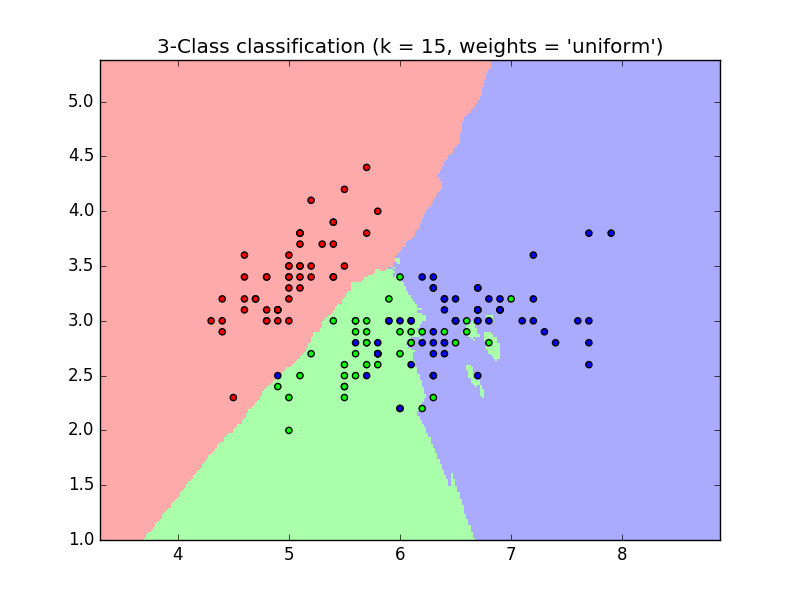
\includegraphics[width=0.7\textwidth]{Figures/knn_schema.png}
	\caption{Visualization of area coverage of three different class membership for kNN classifier with k=15, using euclidean metric. Image taken from \cite{Scikit-Learn_Website}}
	\label{fig:knn_schema}\vspace{-3pt}
\end{figure}

\section{SVM}

Support Vector Machines (SVM) are a~collection of supervised learning methods used for classification, regression and outliers detection. The SVM algorithm relies on a~construction of hyperplane with a~maximal margin that separates patterns of two classes~\cite{CortesVapnik1995}. Creation of the hyper-plane that has the largest distance to the nearest training data points of any class (so-called functional margin) is important since, in general, the larger the margin the lower the generalization error of the classifier.

In SVM's mathematical definition the two classes' labels are denoted as -1 and 1. When treating elements from those sets as points of the Euclidean space $\mathbb{R}^{n}$ (or vectors of this space) the SVM training can be seen as the problem of finding the maximum-margin hyperplane that divides those samples. This issue can be described by formula: \[ w * x - b = 0 \] where $w, x \in \mathbb{R}^{n}, b \in \mathbb{R}$. The $x_{i}$ vectors are samples from the training set, and $w$ is a normal vector to the hyperplane, obtained as a linear combination of those training vectors that lie at borders of the margin: \[ w = \Sigma_{i}\alpha_{i}x_{i} \] Those of the training vectors $x_{i}$ that satisfy the following condition: \[ y_{i}(x * x_{i} - b) = 1\] are called support vectors, and have their corresponding $\alpha_{i} \neq 0$. The $y_{i} \in {-1, 1}$ corresponds to the class labels that training data consists of. The linear decision function used for classifying patterns is expressed as follows: \[I(x) = sgn(\Sigma\alpha_{i}x_{i} * x - b)\] where $\alpha_{i}x_{i} = w_{i}$. SVM efficiency can be enhanced by using different kernel functions which help in solving non-linearly-separable problems. The generalized decision function using kernel function $K$: \[I(x) = sgn(\Sigma\alpha_{i}K(x_{i},x) - b)\]

\begin{figure}[htp]
	\centering
	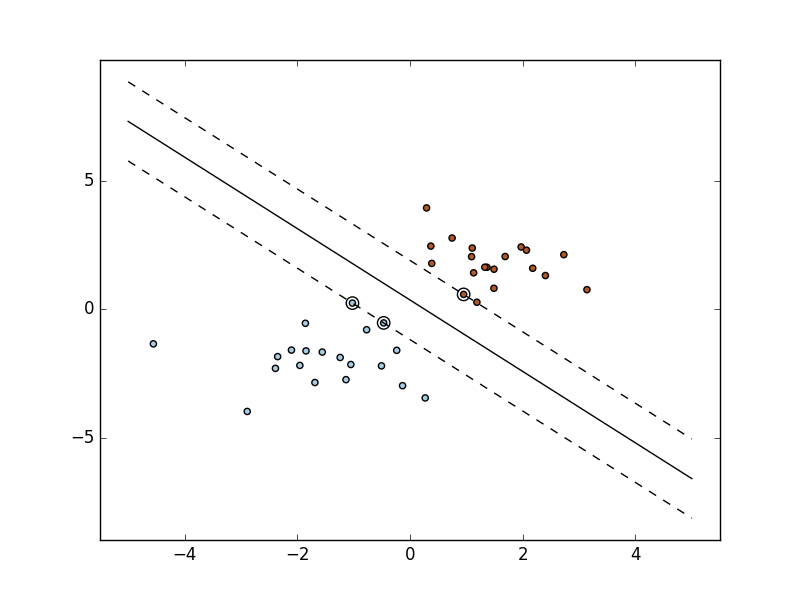
\includegraphics[width=0.7\textwidth]{Figures/svm_hyperplane_margin.png}
	\caption{SVM hyperplane construction with the biggest possible margin for training dataset. Image taken from \cite{Scikit-Learn_Website}}
	\label{fig:svm_hyperplane_margin}\vspace{-3pt}
\end{figure}


\begin{figure}[htp]
	\centering
	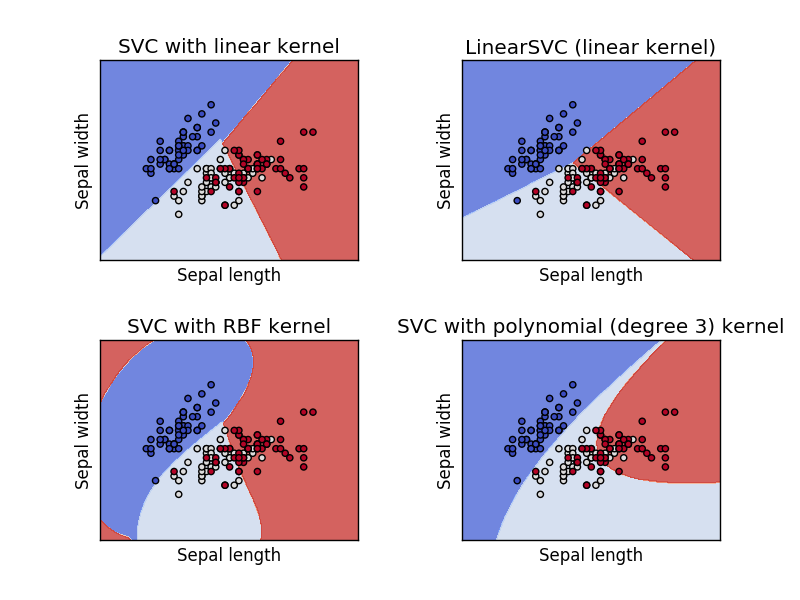
\includegraphics[width=1.0\textwidth]{Figures/svm_kernel_functions.png}
	\caption{Different class area coverages resulting from usage of different kernel functions. Image taken from \cite{Scikit-Learn_Website}}
	\label{fig:svm_kernel_functions}\vspace{-3pt}
\end{figure}

SVMs are effective in high-dimensional spaces, memory efficient, and quite versatile because of the many kernel functions that can be specified for the decision function. Implementation available as part of scikit-learn package lets user specify and tweak many aspects of classifier such as:

\begin{itemize}
	\item $C$ - penalty parameter C of the error term, used to regularize the estimation. If dealing with noisy observations it's recommended to decrease its value
	\item $kernel$ - kernel type used in the algorithm, in this paper one of "poly" or "rbf" values are used. "poly" stands for polynomial kernel using following equation $(\gamma \langle x, x' \rangle + r)^{d}$ (where d is function degree, with default value 3), "rbf" is an acronym for radial basis function with given equation $exp(-\gamma|x - x'|^{2})$
	\item $gamma$ - kernel coefficient for "rbf", "poly" types as can be seen it the kernel equations
	\item $degree$ - degree of the polynomial kernel function
\end{itemize}

It is worth noting though that in some cases, where the number of features is much greater than the number of samples, using support vector machines can give poor results, and is not cost-efficient when calculating probability estimates. 

\section{Random Forest}

\begin{figure}[htp]
	\centering
	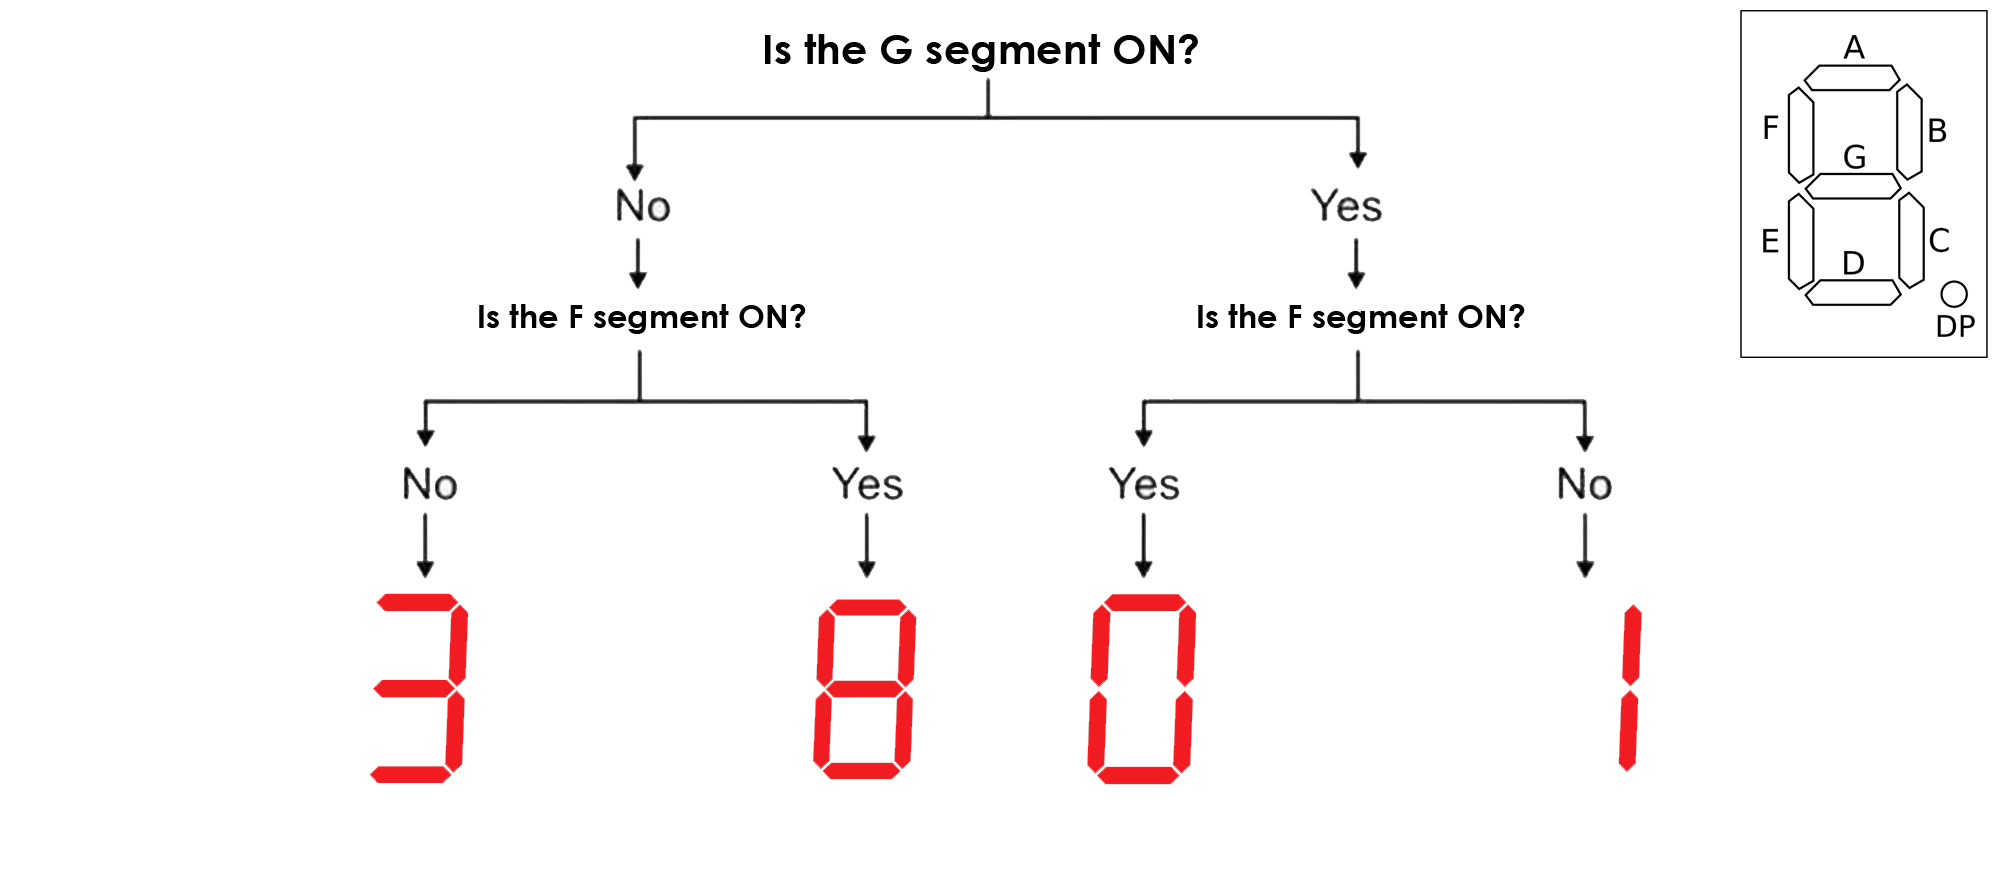
\includegraphics[width=0.8\textwidth]{Figures/rf_visualization_funny.jpg}
	\caption{A funny example of a decision tree}
	\label{fig:rf_visualization_funny}\vspace{-3pt}
\end{figure}

Random forest is a~popular ensemble method. The main principle behind ensemble methods, in general, is that a~group of ``weak learners'' can come together to form a~``strong learner''. In the random forest algorithm~\cite{Breiman2001} the weak learners are decision trees, which are used to predict class labels. A decision tree is a decision support tool that uses a tree-like graph for classification issue. Each graph node performs a test on an attribute of the provided pattern and sends it to its child node via a branch that represents the outcome of the test. Each leaf in a decision tree represents a certain class label. In other words for a~feature vector representing one pattern a~decision tree calculates its class label by dividing value space into two or more subspaces. More precisely, an input data is entered at the top of the tree and as it traverses down the tree the data gets bucketed into smaller subsets. There are many advantages of using decision trees. Their results are easy to interpret and visualize in form of a graph, they can handle multi class classification problems and perform well even if its assumptions are somewhat violated by the true model from which the data were generated. On the other hand, the main drawbacks connected to their usage consist of overfitting problem caused by creating too complex trees on a very complicated data, and instability caused by small variations in the data that might result in a completely different tree being generated. That last problem is easily mitigated by ensembling set of decision trees into a random forest. 

\begin{figure}[htp]
	\centering
	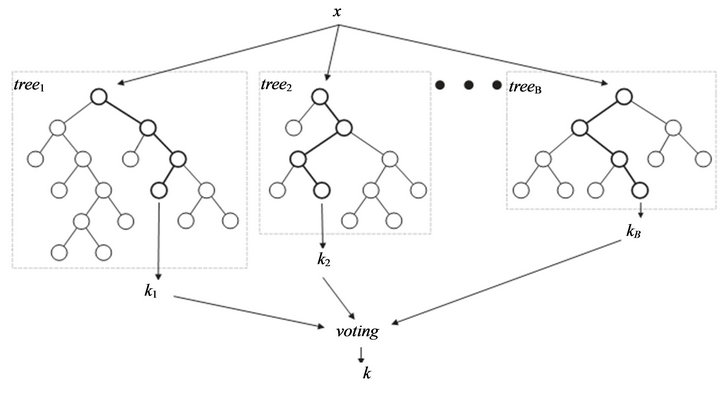
\includegraphics[width=0.85\textwidth]{Figures/rf_visualization.jpg}
	\caption{Visualization of a random forest consisting of $B$ different decision trees}
	\label{fig:rf_visualization}\vspace{-3pt}
\end{figure}

In the random forest a~large number of classification trees is formed, which altogether serve as a~classifier. In order to grow each tree, a~random selection of rows from the training set is drawn. Random sampling with replacement is also called bootstrap sampling. In addition, when constructing trees for a~random forest at each node $m$~variables out of the set of all input variables are randomly selected, and the best split on these $m$~is used to split the node. After a~relatively large number of trees is generated, they vote for the most popular class. Some of the parameters used for improving classification rates that are available within scikit-learn package random forest implementation:

\begin{itemize}
	\item $n\_estimators$ - determines number of trees used by random forest in the algorithm
	\item $max\_depth$ - the maximum depth of each tree in the forest
	\item $max\_features$ - the number of features to consider when looking for the best split
	\item $min\_samples\_leaf$ - the minimum number of samples required to be at a leaf node
\end{itemize}

Random forests join few important benefits: (a)~they are relatively prone to the influence of outliers, (b)~they have an embedded ability of feature selection, (c)~they are prone to missing values, and (d)~they are prone to over-fitting.